The probability hypothesis density (PHD) function is the first-order moment of a random finite set, also known as the \textit{intensity function}. Its value is the expected number of targets in a certain area of the target space. From Section \ref{sec:prob-distributions}, we know that the first-order moment is the expectation value, but what is the expectation value of a set? To answer this question, let us define the problem formally. The computations that follow are based on the original book by Mahler \cite[576--578]{mahlerStatisticalMultisourcemultitargetInformation2007}.

Let a random finite set be denoted by $\Xi$ with the multi-target probability distribution $p_\Xi(X)$, and the target space $\mathcal{X}$. The expected number of targets is, conceptually, the integral over all targets multiplied by the value of the probability density function for each state value. However, since summing over targets will not have any meaning in terms of the expected value, we introduce the delta function of a set:

\begin{equation}
    \delta_\Xi(\mathbf{x}) = \begin{cases}
        0 & \text{if } X = \emptyset, \\
        \sum_{\mathbf{w} \in X} \delta_\mathbf{w}(\mathbf{x}) & \text{otherwise},
    \end{cases}
\end{equation}

\noindent where $\delta_\mathbf{w}$ is the Dirac delta density centered at $\mathbf{w}$, the continuous-space analog of the Kronecker delta function mentioned in Definition \ref{def:cardinality-rfs}.

\begin{definition}[PHD function]\label{def:phd-function}
    Given a random finite set $\Xi$, where elements of $\Xi$ are from $\mathcal{X}$, with the multi-target density $p_\Xi(X)$, the expected value of the set $\Xi$ is defined as:

    \begin{equation}
        v_\Xi(\mathbf{x}) = E[\delta_\Xi(\mathbf{x})] = \int \delta_\Xi(\mathbf{x}) \cdot p_\Xi(X) \delta X.
    \end{equation}

    \noindent The function $v_\Xi(\mathbf{x})$ is also called the Probability hypothesis density (PHD) function.
\end{definition}

The PHD function is not a probability density function, that is, it is not normalized to integrate to one. The integral of the PHD function over some subspace $S$ yields the expected number of targets in this subspace:

\begin{equation}\label{eq:phd-func-integral}
    E[| \Xi \cap S |] = \int_S v_\Xi(\mathbf{x}) \mathrm{d} \mathbf{x}.
\end{equation}

This formulation prompts that the PDF function is an unnormalized multi-target probability density function with the normalization constant equal to the expected number of existing targets $\hat{N}$ over the whole space $\mathcal{X}$, i.e., $\hat{N} = \int_\mathcal{X} v_\Xi(\mathbf{x}) \mathrm{d} \mathbf{x}$. Therefore, the peaks of this distribution are the most probable locations of the tracked targets. The density evolves over time as targets move in space. An example of the PHD function is illustrated in Figure \ref{fig:phd-function}.

\begin{figure}
    \centering
    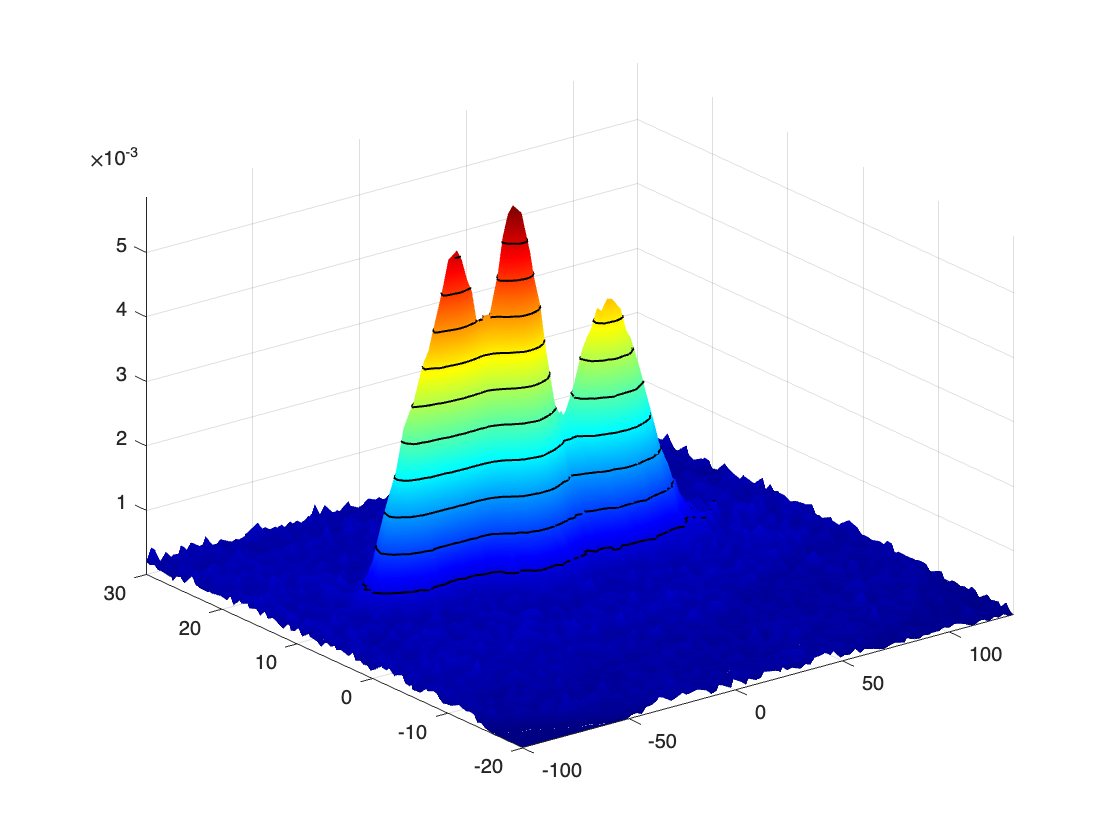
\includegraphics[width=.6\linewidth]{figures/phd-function.png}
    \caption[PHD function example.]{An example of the PHD function. Three targets move in the 2D Euclidean space according to a CV model. Note that this function is not normalized, which means that the integral over the entire space is not equal to one. In this example, the expected number of targets in the space is approximately 3.2245, which can be inferred from the location of the corresponding peaks.}
    \label{fig:phd-function}
\end{figure}

The fact that the PHD function does not include normalization allows an efficient computation of this function in terms of the computational complexity. This fundamental property of the PHD function led to the development of the PHD filter. In the next section, we will define several assumptions of the PHD filter and define the predict-update cycle.
